%! Author = impy
%! Date = 30/05/2020

% Preamble
\documentclass[11pt]{article}

% Packages
\documentclass{article}
\usepackage{amsmath,amsthm,amssymb}
\usepackage{mathtext}
\usepackage[T1,T2A]{fontenc}
\usepackage[utf8]{inputenc}
\usepackage[english,russian]{babel}
\usepackage{graphicx}
\usepackage{tikz}
%\usepackage{xcolor}
%\usepackage{hyperref}
\graphicspath{{../../graphics/}}

\title{Лабораторная работа No1.
Часть I Методы одномерного поиска экстремума}
\author{Торопин Константин}
\date{May 2020}


% Document

\begin{document}

    \maketitle

    \section{Постановка задачи}

    Для реализации одномерного поиска экстремума функции были написаны 3 алгоритма:
    \begin{enumerate}
        \item Метод дихотомии (деления отрезка пополам)
        \item Метод золотого сечения
        \item Метод Фибоначчи
    \end{enumerate}

    Функция для анализа была взята - $x^2 + 2x - 4, x \in [-10,20]$ \\
    Заметим что минимум этой функции = 5 при значении $x = -1$ \\
    Для тестирования алгоритмов параметр $\epsilon$ был выбран равным $10^{-5}$\\

    Так же реализованы алгоритм поиска минимума функции на прямой и алгоритм минимизации функции переменных в направлении заданного вектора. \\
    Весь код находится по ссылке - \href{https://github.com/ImpyAngel/metOpt/blob/master/lab1.py}


    \section{Выводы}

    Исходя из полученных данных можно увидеть что метод дихотомии справляется с задачей медленнее чем методы золотого сечения и Фибоначчи. \\
    Однако метод Фибоначчи на первых этапах итераций сходится куда медленнее чем другие методы. \\
    Что касается анализа скорости работы алгоритмов для достижения нужной точности, то здесь все методы показывают близкий к линейному росту в зависимости от логарифма нужной точности.
    Что и выводится исходя из теории.
    Наиболее быстрый по сходимости оказывается метод золотого сечения.
    График метода фибоначчи показывает наиболее линейный рост.

    \section{Графики}

    \begin{figure}[h]
        \begin{minipage}[h]{0.47\linewidth}
            \center{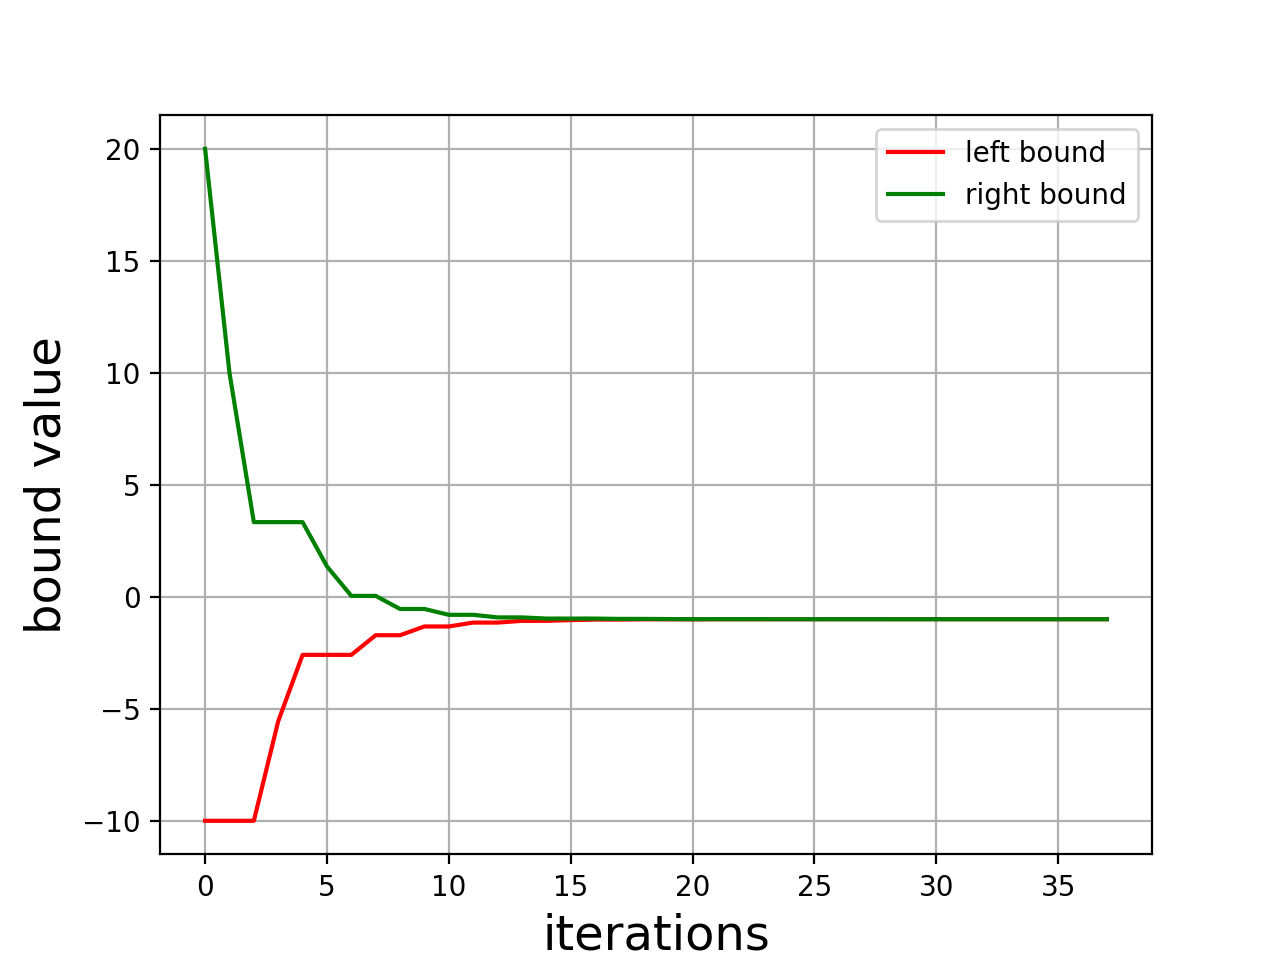
\includegraphics[width=1\linewidth]{dichotomy_bounds_30-05-01:59:14.png}}  Метод дихотомии \\
        \end{minipage}
        \hfill
        \begin{minipage}[h]{0.47\linewidth}
            \center{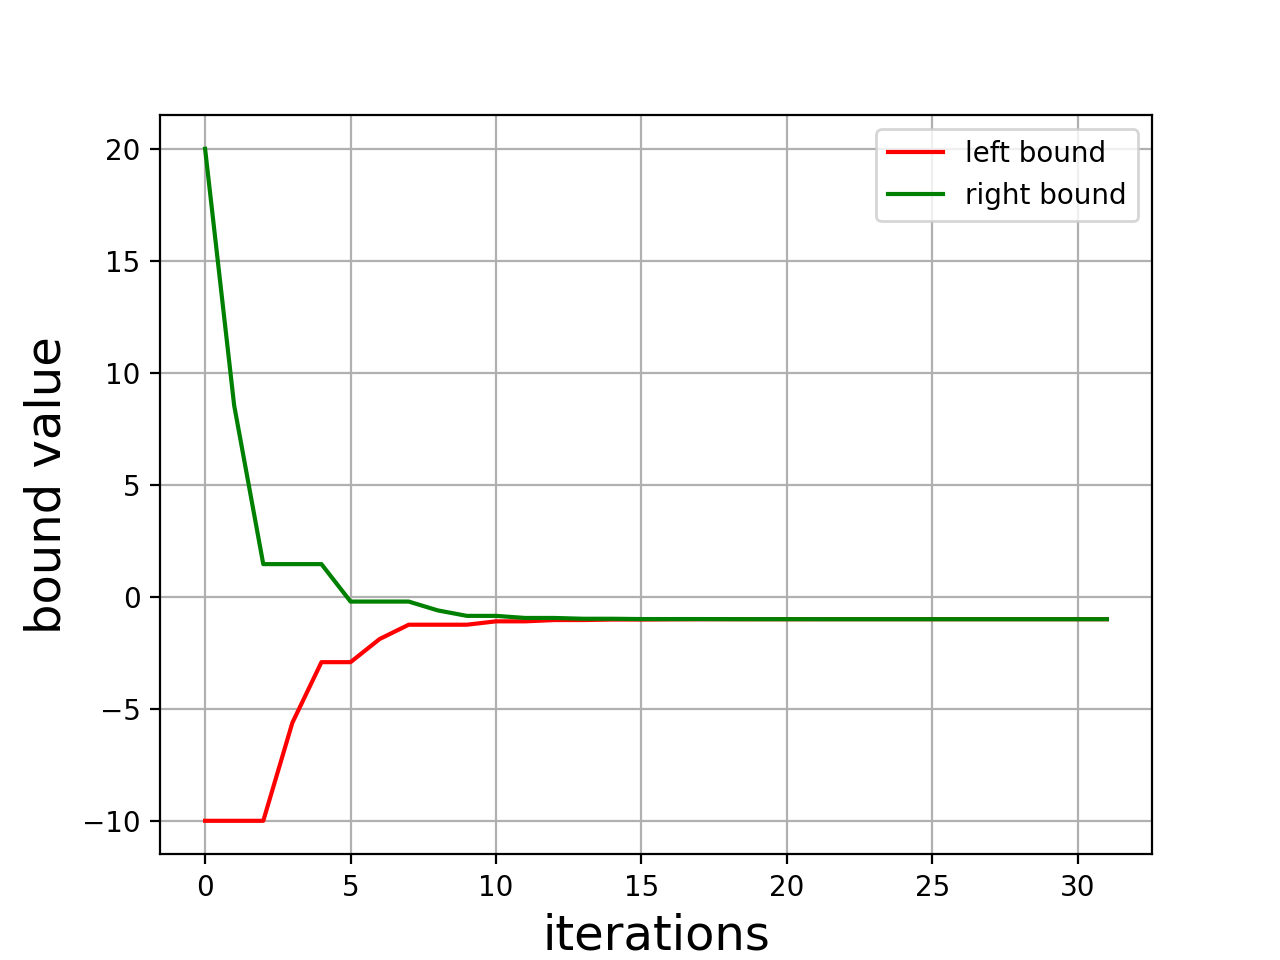
\includegraphics[width=1\linewidth]{golden_ratio_bounds_30-05-01:59:16.png}} \\Метод золотого сечения
        \end{minipage}
        \vfill
        \center
        \begin{minipage}[h]{0.47\linewidth}
            \center{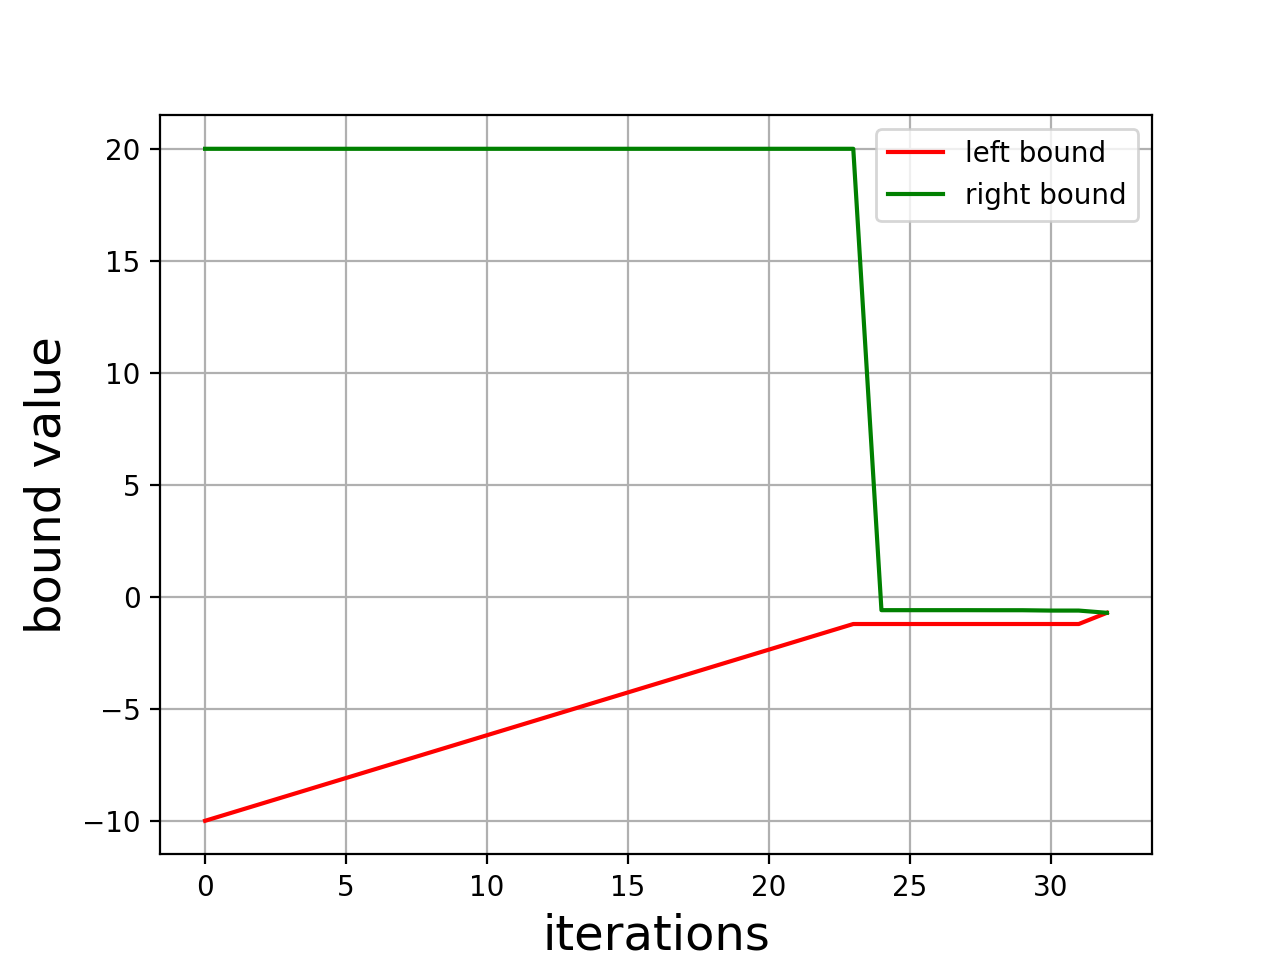
\includegraphics[width=1\linewidth]{mem_fib_bounds_30-05-01:59:17.png}} Метод Фибоначчи \\
        \end{minipage}
        \caption{В первом случае был рассмотрен анализ поведения левой и нижней границы в которых лежит значение минимума функции}
        \label{ris:experimentalcorrelationsignals}
    \end{figure}

    \begin{figure}[h]
        \begin{minipage}[h]{0.47\linewidth}
            \center{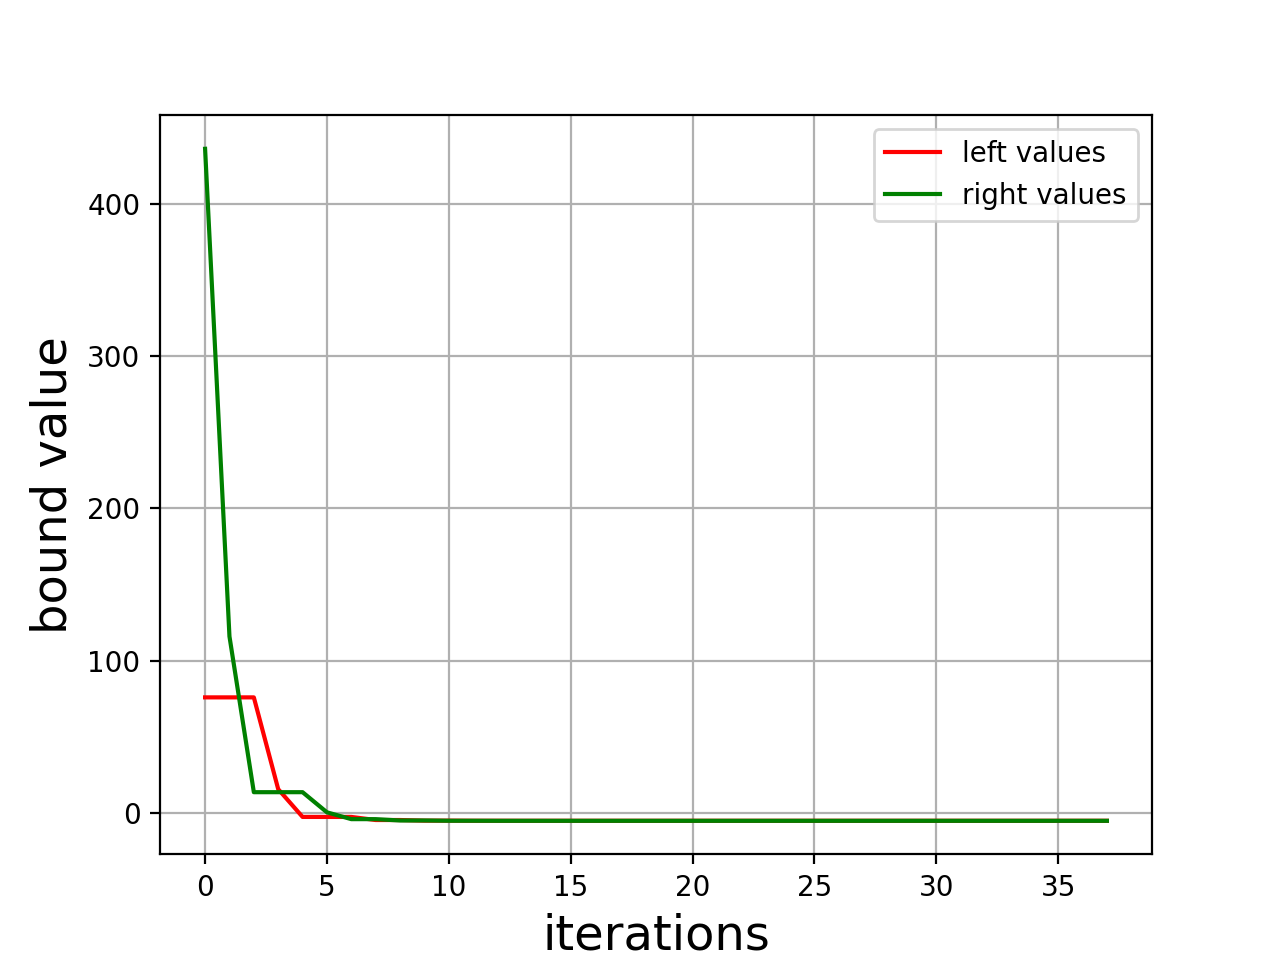
\includegraphics[width=1\linewidth]{dichotomy_bound_values_30-05-01:59:14.png}}  Метод дихотомии \\
        \end{minipage}
        \hfill
        \begin{minipage}[h]{0.47\linewidth}
            \center{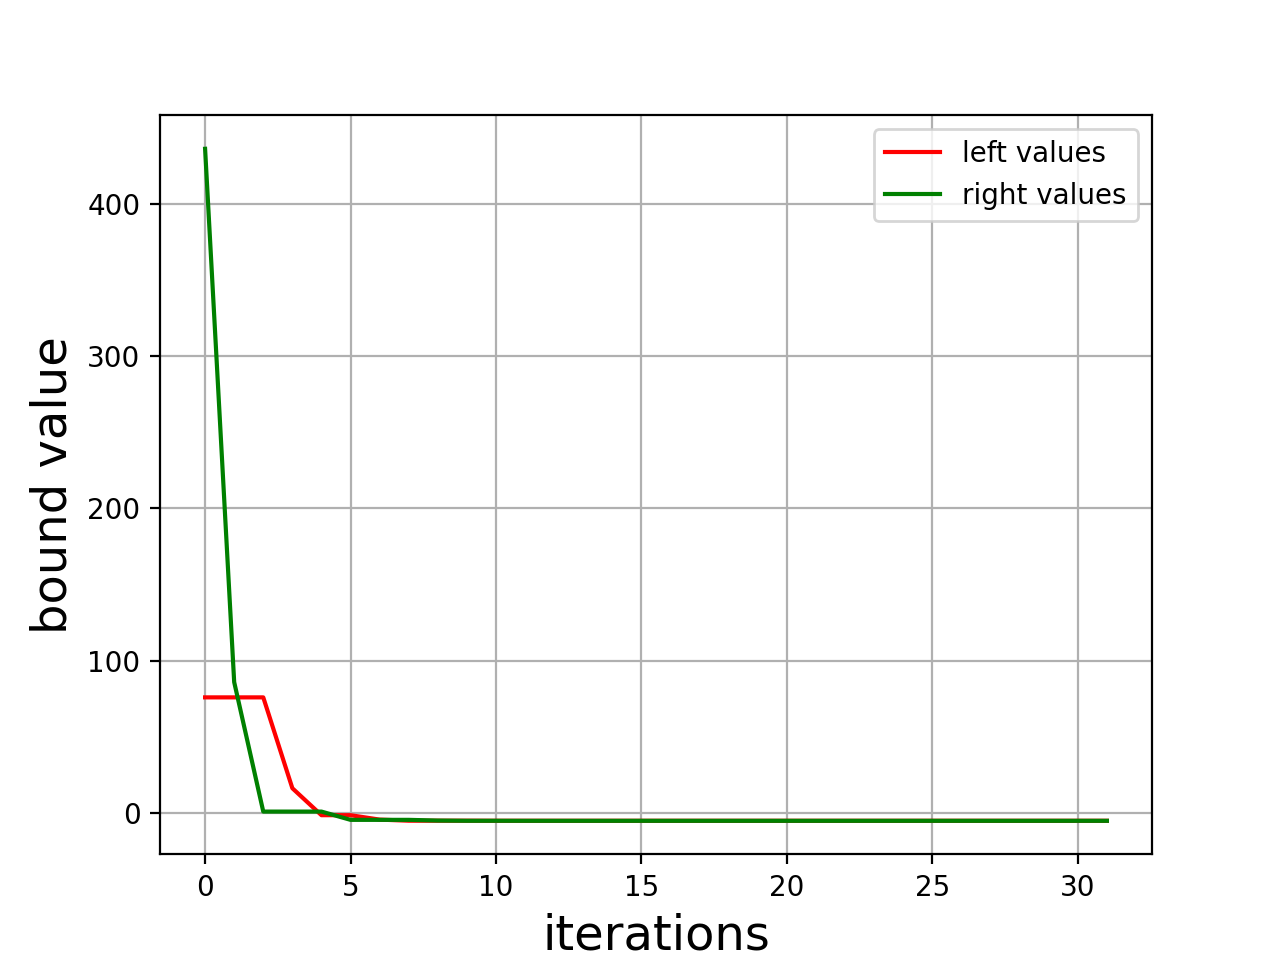
\includegraphics[width=1\linewidth]{golden_ratio_bound_values_30-05-01:59:16.png}}\\Метод золотого сечения
        \end{minipage}
        \vfill
        \center
        \begin{minipage}[h]{0.47\linewidth}
            \center{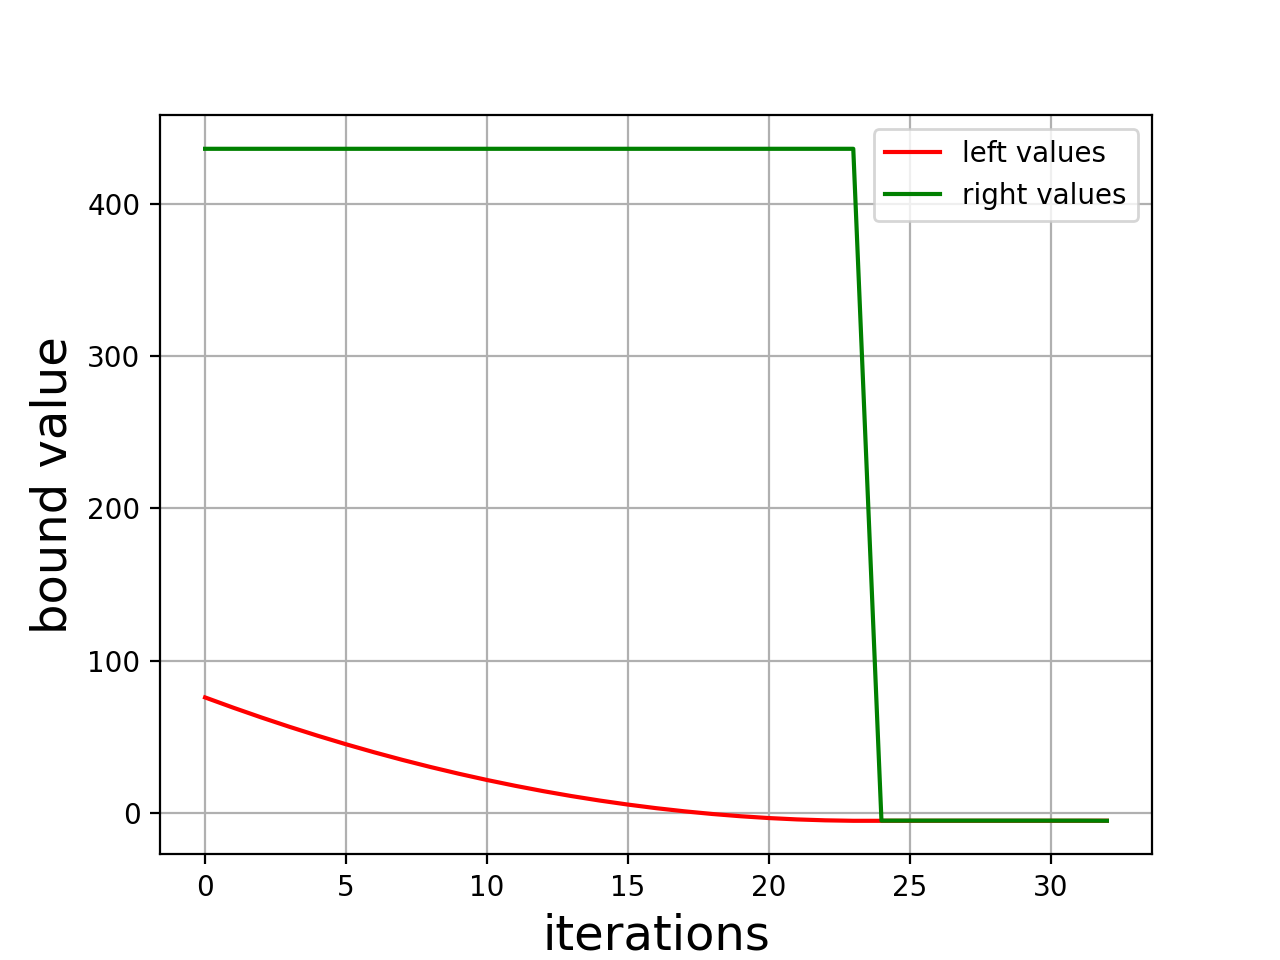
\includegraphics[width=1\linewidth]{mem_fib_bound_values_30-05-01:59:17.png}} Метод Фибоначчи \\
        \end{minipage}
        \caption{Графики значения функции на этих границах}
    \end{figure}


    \begin{figure}[h]
        \begin{minipage}[h]{0.47\linewidth}
            \center{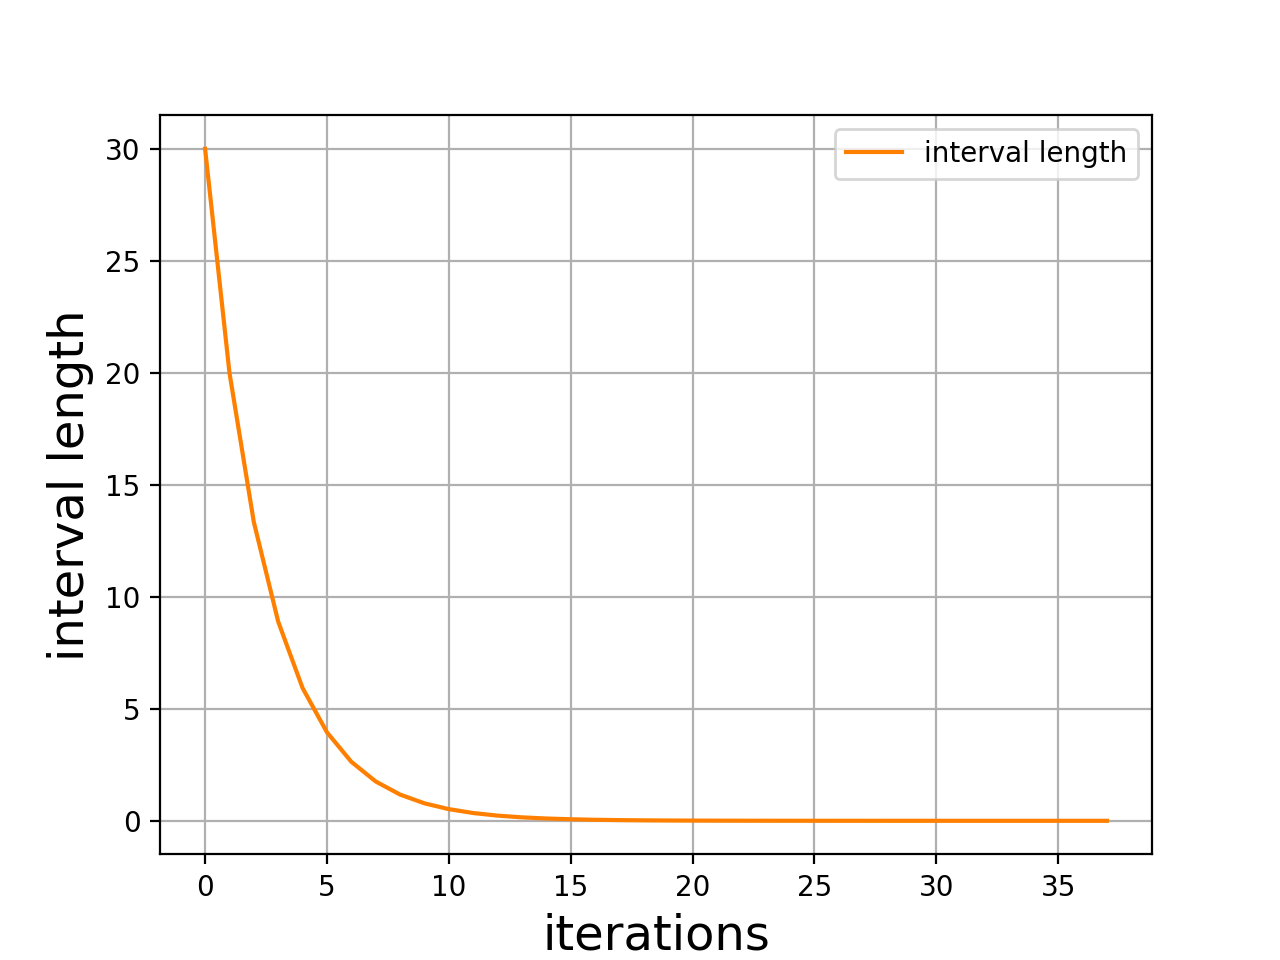
\includegraphics[width=1\linewidth]{dichotomy_bound_len_30-05-01:59:15.png}}  Метод дихотомии \\
        \end{minipage}
        \hfill
        \begin{minipage}[h]{0.47\linewidth}
            \center{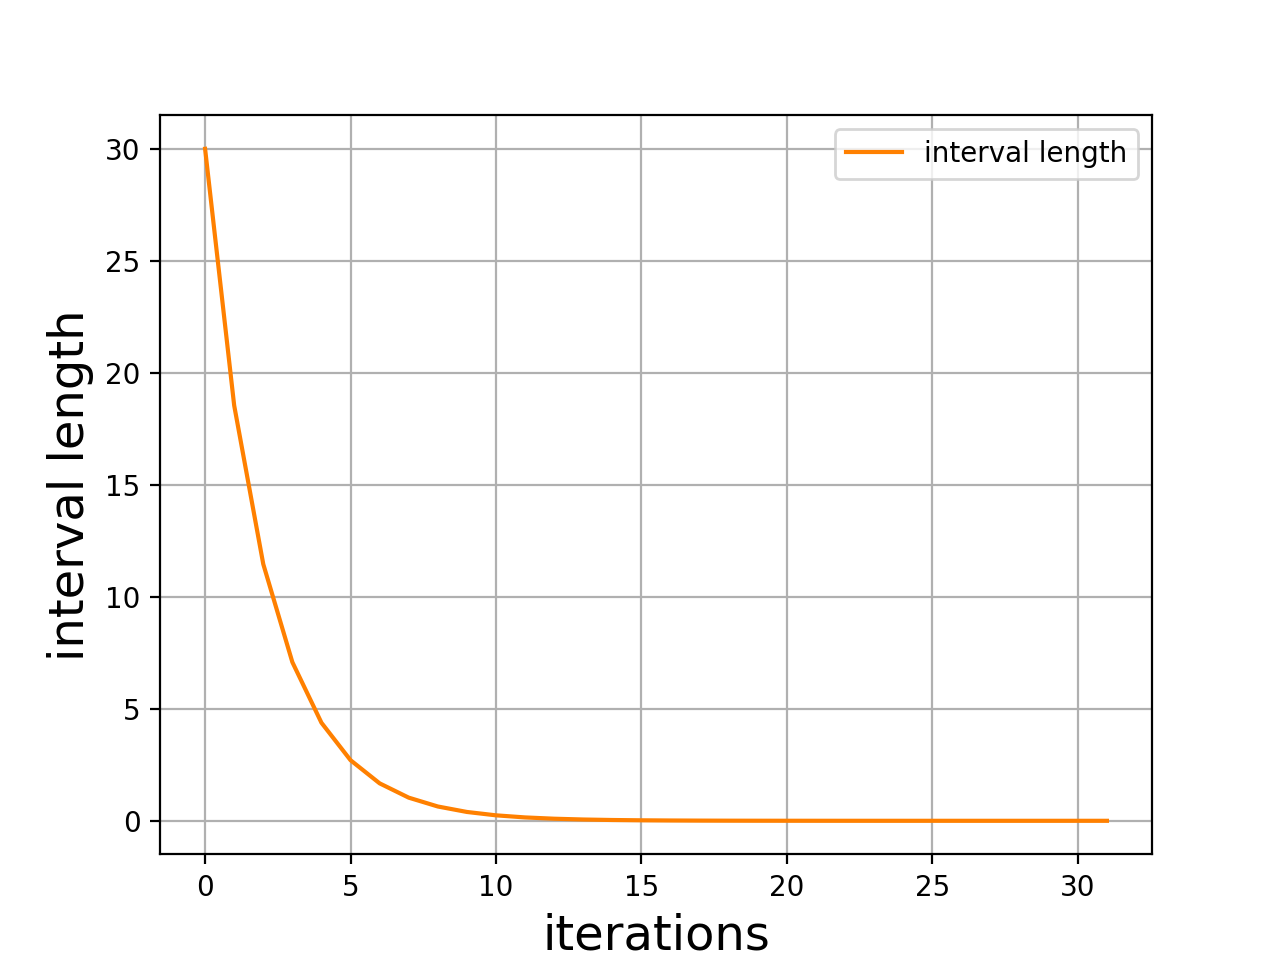
\includegraphics[width=1\linewidth]{golden_ratio_bound_len_30-05-01:59:16.png}}\\Метод золотого сечения
        \end{minipage}
        \vfill
        \center
        \begin{minipage}[h]{0.47\linewidth}
            \center{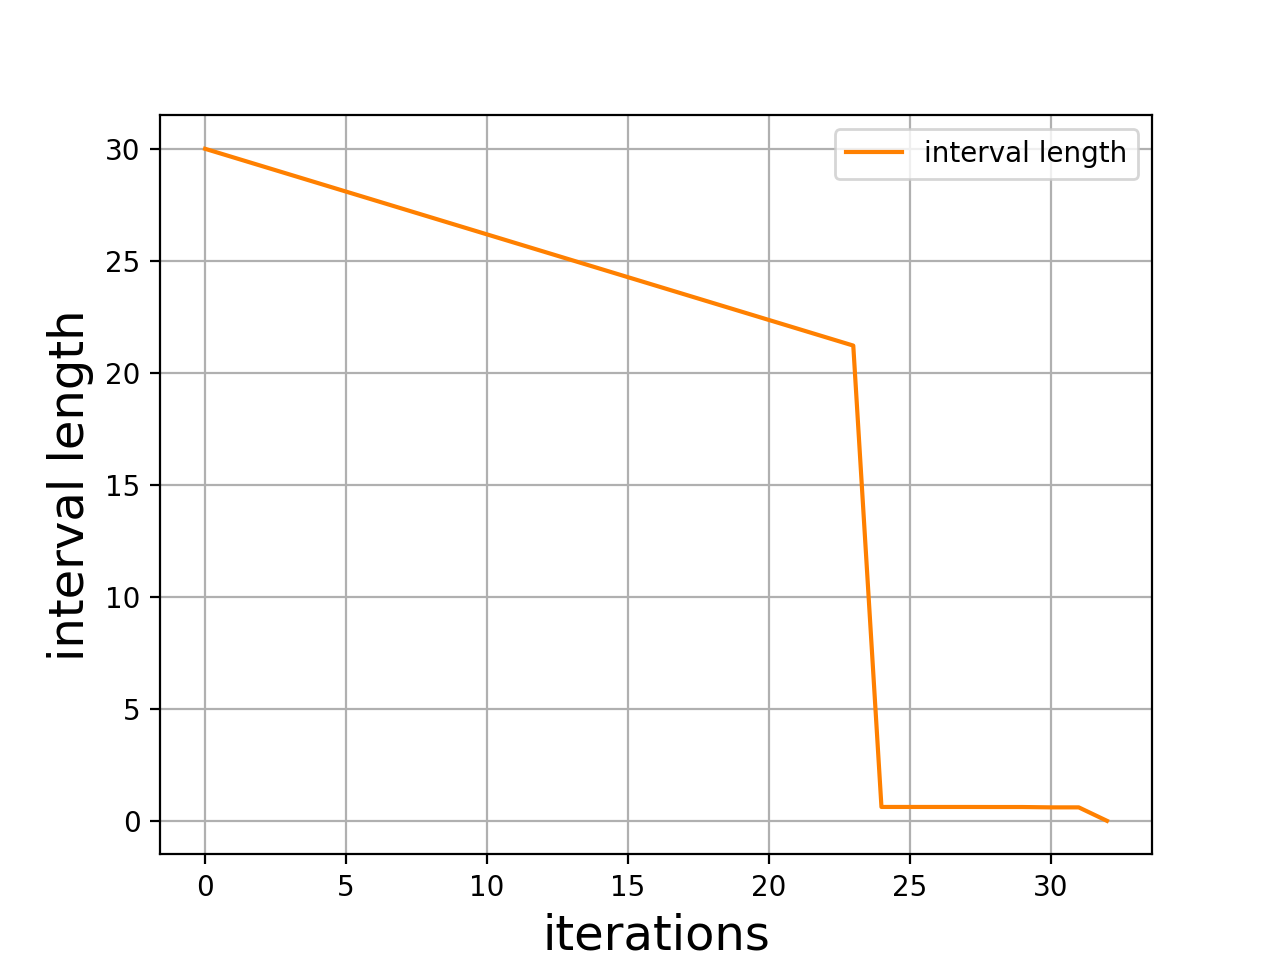
\includegraphics[width=1\linewidth]{mem_fib_bound_len_30-05-01:59:18.png}} Метод Фибоначчи \\
        \end{minipage}
        \caption{Графики отношения размера границ с итерациями}
    \end{figure}

    \begin{figure}[h]
        \begin{minipage}[h]{0.47\linewidth}
            \center{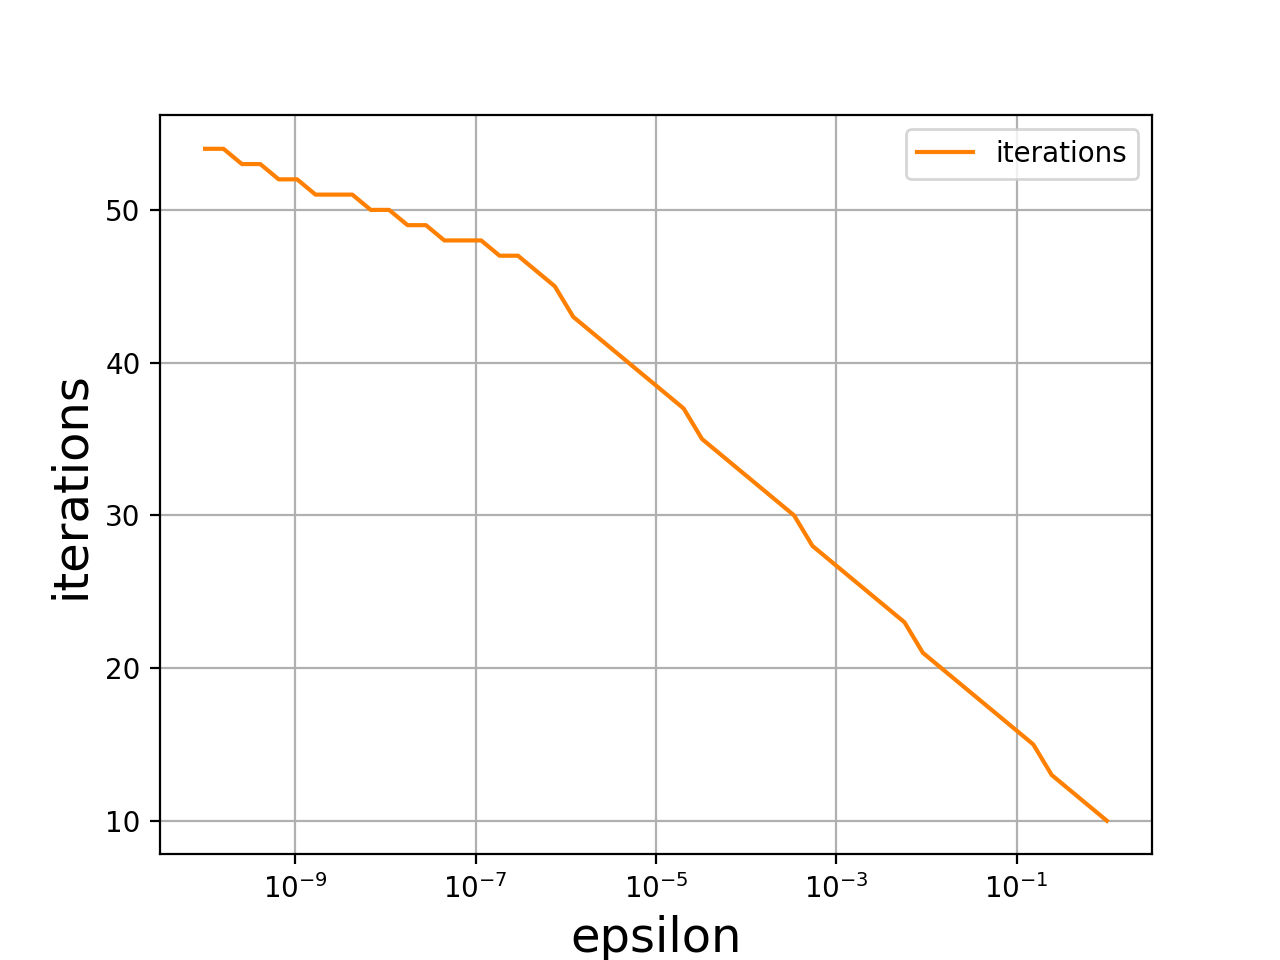
\includegraphics[width=1\linewidth]{dichotomy_log_eps_iters_30-05-01:59:15.png}}  Метод дихотомии \\
        \end{minipage}
        \hfill
        \begin{minipage}[h]{0.47\linewidth}
            \center{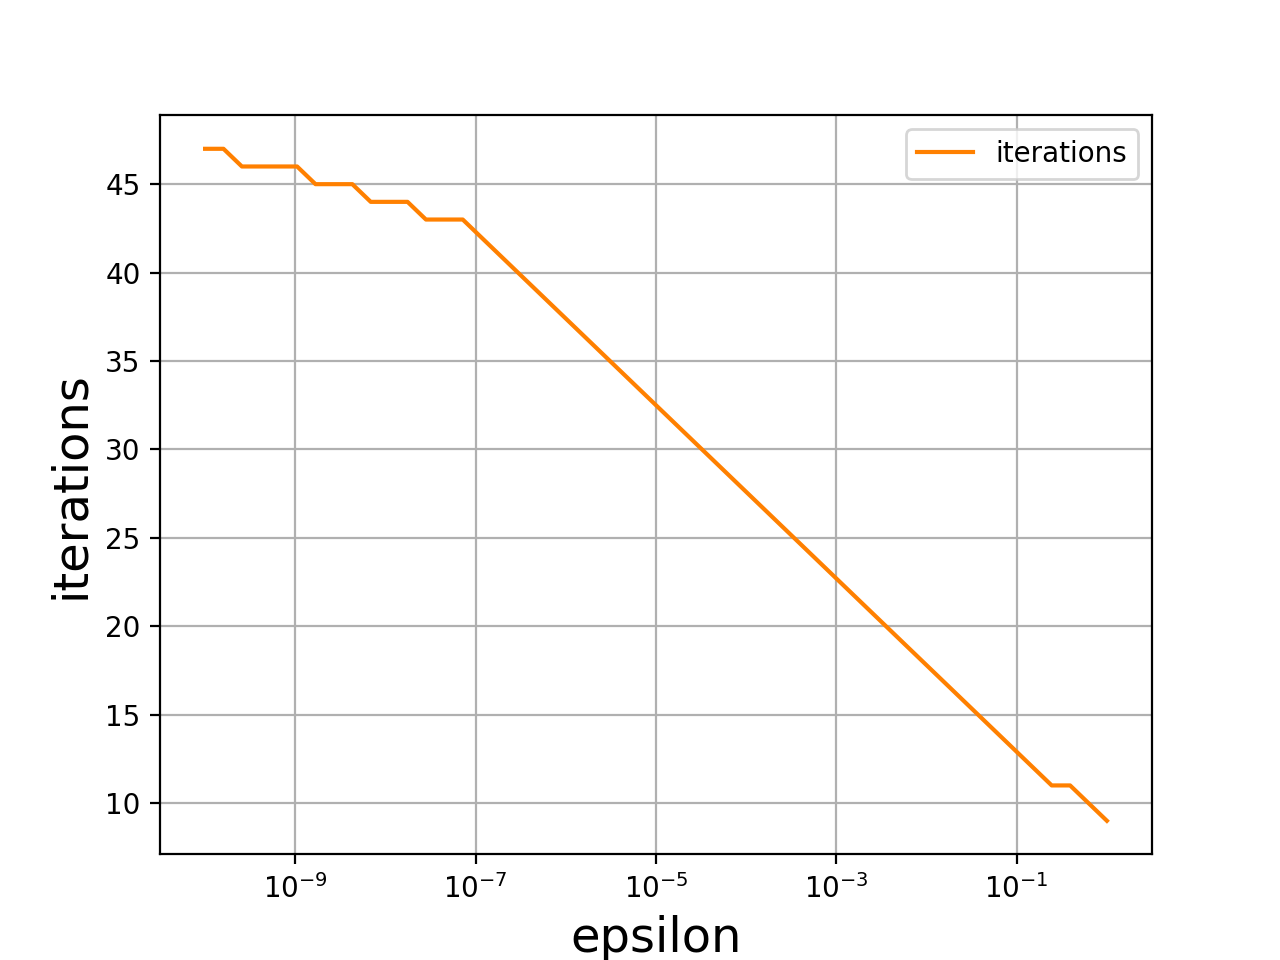
\includegraphics[width=1\linewidth]{golden_ratio_log_eps_iters_30-05-01:59:17.png}}\\Метод золотого сечения
        \end{minipage}
        \vfill
        \center
        \begin{minipage}[h]{0.47\linewidth}
            \center{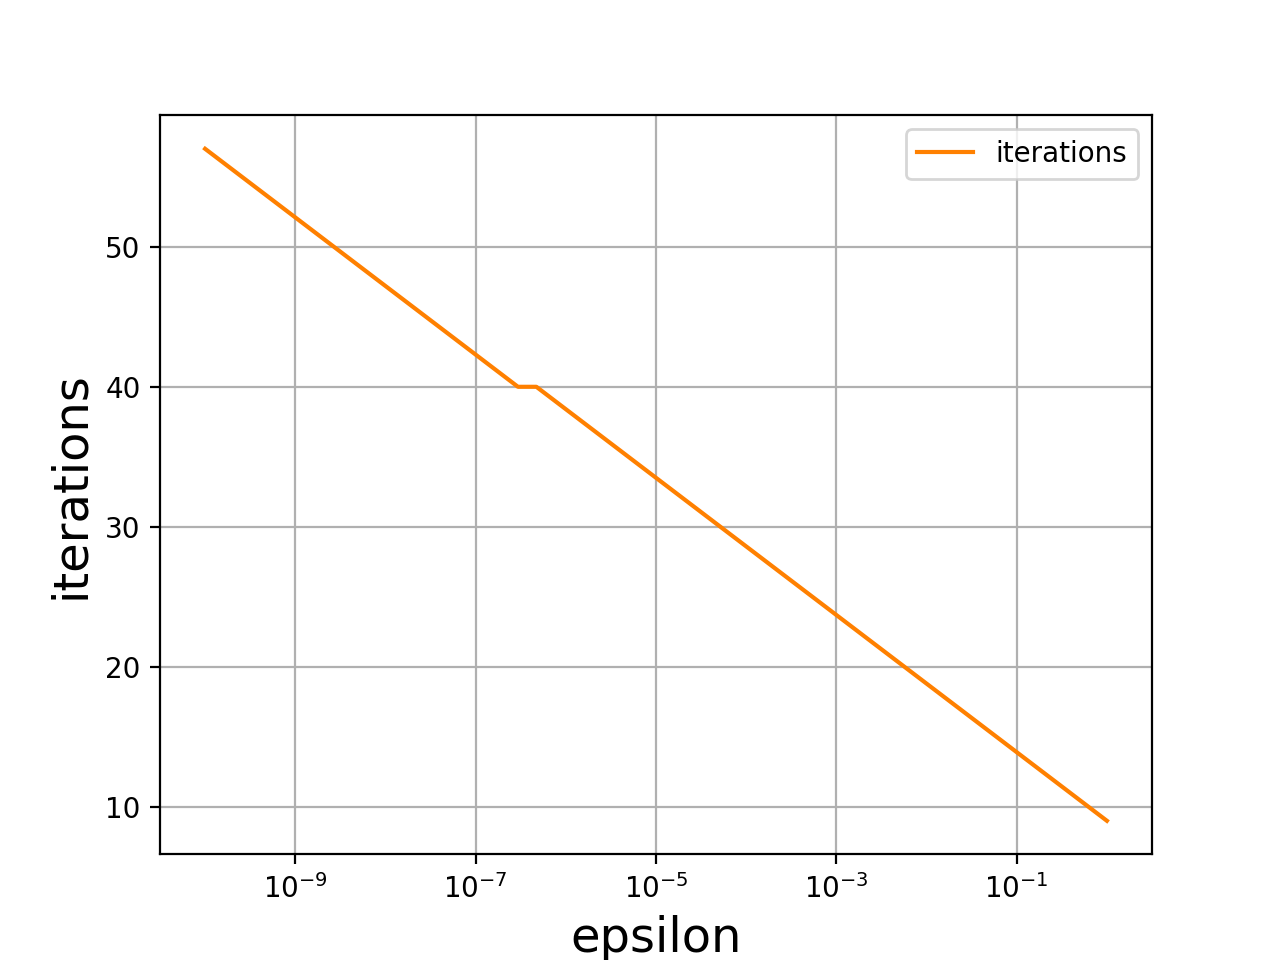
\includegraphics[width=1\linewidth]{mem_fib_log_eps_iters_30-05-01:59:18.png}} Метод Фибоначчи \\
        \end{minipage}
        \caption{Далее рассмотрен процесс изменения количества итераций нужных для достижения конкретной точности - $\epsilon$ \\
            Значения $\epsilon$ изменялось в интервале $[10^{-10}, 1]$ с логарифмичном шагом.}
    \end{figure}

\end{document}